\documentclass[11pt]{article}
\usepackage[letterpaper,margin=.72in]{geometry}
\usepackage[T1]{fontenc}
\usepackage{lmodern,microtype,graphicx,booktabs,amsmath,hyperref}
\hypersetup{colorlinks=true,urlcolor=blue,pdfauthor={James N. Jean IV},pdftitle={Recorded departure transfer with held station geography}}
\setlength{\parindent}{0pt}\setlength{\parskip}{6pt}\renewcommand{\arraystretch}{1.1}
\begin{document}
{\Large\bfseries Recorded departure transfer with held station geography}\par
James N. Jean IV\hfill 29 October 2026\par
\textit{Independent study 06. Not peer reviewed.}
\section*{Decision brief}
Can geographical pooling transfer recorded departure counts when a station history is withheld? This fixed retrospective comparison uses published 2024 departure rows and initial-quarter coordinate medians. It simulates cold start on previously observed station IDs; it does not verify actual openings, relocations, bike stock or dock availability.

Conditional finding. Across 12 held coordinate groups and 2,208 station-days, geographic MAE is 11.621 departures/day versus 21.047 for a pooled weekday baseline, a 44.8\% reduction. Two groups have higher errors. Temporal settings also differ between the selected model and baseline, so the comparison does not isolate geography's contribution. All 54 validation candidates and the full held stress grid remain available.

Next evidence. Test count transfer prospectively only after verifying station identity, geometry and input vintages. Immediate complete prior-day donor counts are an idealized assumption; the public files were posted later. Obtain stock, availability and opening/relocation telemetry before a rebalancing decision. No operational benefit or realized savings is established.

\begin{center}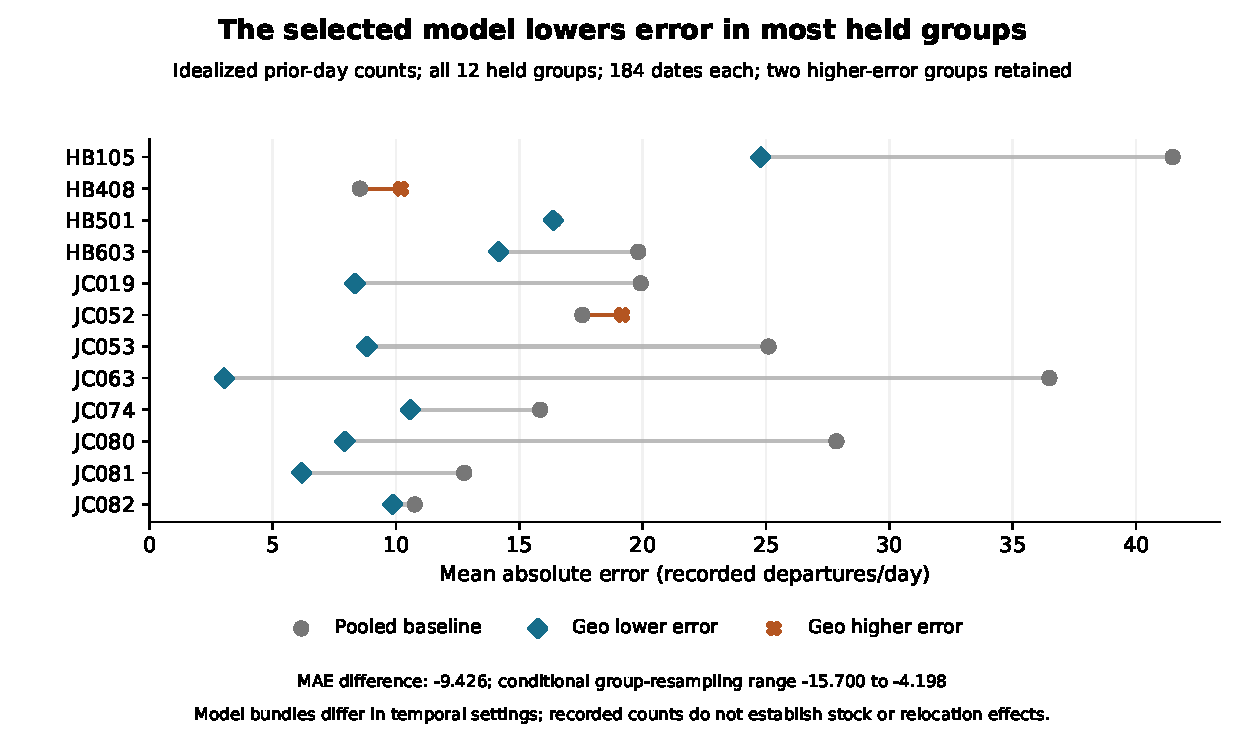
\includegraphics[width=\linewidth]{images/held_group_errors.pdf}\end{center}
\small Figure 1. Every held group is shown. HB408 and JC052 have higher geographic-model errors. The resampling range conditions on these same twelve proxy groups and is not a guarantee for future sites.\normalsize\par

\newpage\section*{1. Fixed source and grouped geography}
The source is the twelve official JC-2024 monthly files linked by the provider [1,2], totaling 37,273,638 compressed bytes and 1,052,451 published rows. Analysis reads only started\_at, start\_station\_id, start\_lat and start\_lng. Whole-file/member hashes, selected-field parser hashes and all exclusions are retained. Independent pandas versus standard-CSV parsing matches 4,209,804 selected-field scalars; projection/geometry checks cover 92,152 exact fields and 99 radii at fixed tolerance. Coarse grid/control checks add 91,490.

Of 99 initial-quarter nominal IDs, 83 pass the fixed activity/coordinate screens; sixteen are excluded before forecast scoring. The derived grid has 30,378 civil station-days. Zero means zero published departure rows, not an open station or zero latent demand. Source controls establish consistency of the captured publication, not unique rides or true demand. Public facts are purpose-bound coarse derivatives; raw archives and customer/trajectory attributes remain private.

\begin{center}\small\setlength{\tabcolsep}{4pt}
\begin{tabular}{rrrl}\toprule
Fold & Station IDs & Coordinate groups & Role \\
\midrule
0 & 24 & 24 & Donor \\
1 & 12 & 12 & Donor \\
2 & 13 & 12 & Donor \\
3 & 22 & 22 & Validation \\
4 & 12 & 12 & Held \\
\bottomrule\end{tabular}\end{center}
\begin{center}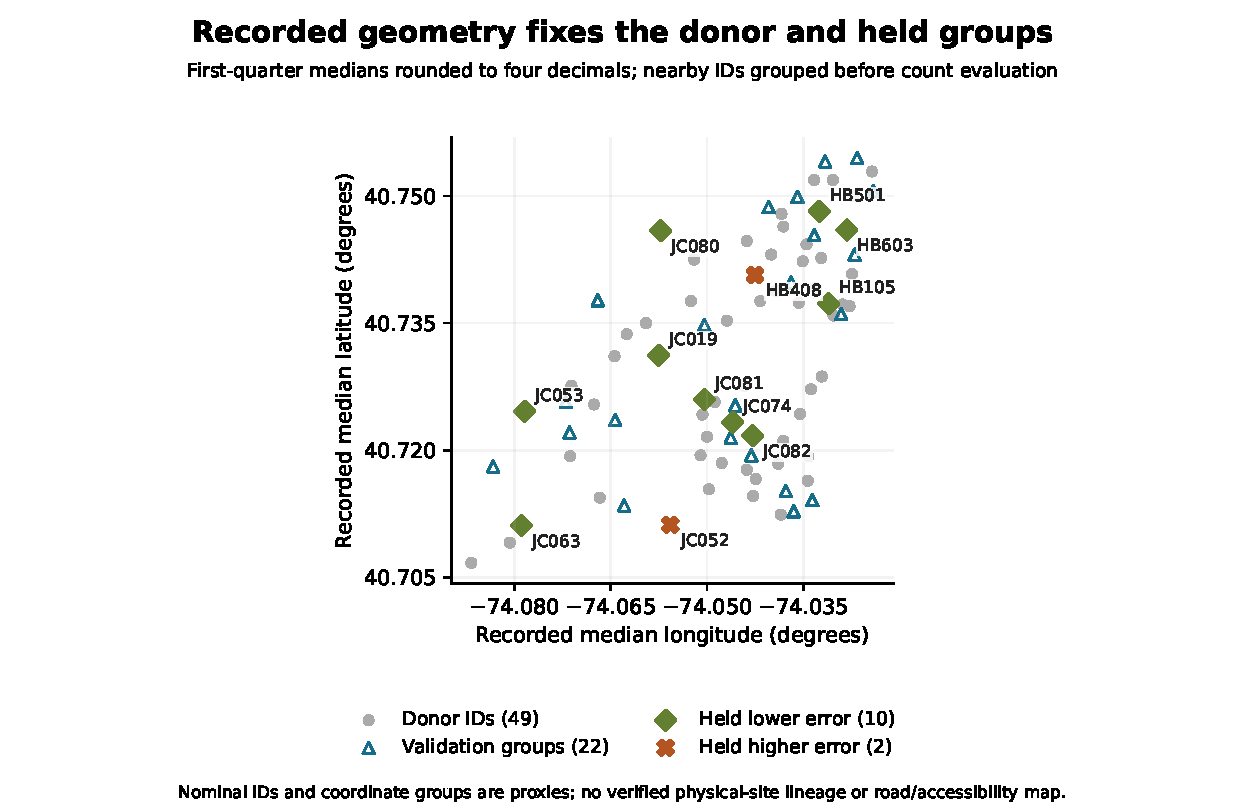
\includegraphics[width=.93\linewidth]{images/coordinate_groups.pdf}\end{center}
\small Figure 2. Initial-only recorded medians define nearby-ID groups and folds. Labels identify every held ID. The grouping is a proxy for related coordinates, not verified physical-site lineage or a road/accessibility map.\normalsize\par

\newpage\section*{2. Actual method and complete validation search}
The protocol was committed at 2205241 before trip retrieval; exact headers were recorded at 55e43a4 before values. Initial eligibility requires activity in January, February and March, at least 95\% valid regional coordinates and a nearest-rank 95th-percentile radius no larger than 150 m around unrounded coordinate medians. Medians are rounded to four decimals for model/public use. These are untuned design screens, not validated physical thresholds. Connected components within 100 m proxy nearby IDs; a fixed SHA-256 rule assigns folds.

Donor folds 0--2 supply only dates before each target. Validation uses fold 3 on April 1--June 30; held uses fold 4 on July 1--December 31. Withheld count histories never enter predictors. Their initial coordinates/activity were observed, making this a simulated count-history holdout rather than proof about a genuinely unopened site. Raw source inputs and quality were visible without blinding.

Each donor mean uses the past 28, 56 or 84 civil days, matched by weekday or weekday/weekend, with at least three matching dates. Average the nearest 3, 5 or 10 donors, using inverse-distance exponents 0, 1 or 2 and a 100 m distance floor [4]. Distances use a 6371 km spherical radius, not road distance. The pooled baseline averages every donor using an 84-day same-weekday history. No embedding or parameter optimizer is executed.

The 54 exploratory configurations are inherited finite choices; they are not an exhaustive optimum. Select equal-coordinate-group validation MAE, breaking exact exported-score ties by smaller neighbor count, lower exponent, shorter window, then weekday. The table includes every candidate MAE; all MSE/RMSE, group and month metrics remain in the exports.

\begin{center}\small\setlength{\tabcolsep}{4pt}
\begin{tabular}{lrrrrr}\toprule
Calendar & k & Exponent & 28 days & 56 days & 84 days \\
\midrule
Weekday & 3 & 0 & 21.343 & 20.841 & 20.747 \\
Weekday & 3 & 1 & 21.566 & 21.042 & 20.928 \\
Weekday & 3 & 2 & 21.804 & 21.232 & 21.097 \\
Weekday & 5 & 0 & 20.563 & 20.116 & 20.151 \\
Weekday & 5 & 1 & 20.495 & 20.071 & 20.108 \\
Weekday & 5 & 2 & 20.917 & 20.466 & 20.481 \\
Weekday & 10 & 0 & 21.407 & 20.918 & 20.872 \\
Weekday & 10 & 1 & 20.908 & 20.478 & 20.469 \\
Weekday & 10 & 2 & 20.972 & 20.519 & 20.520 \\
Weekday/weekend & 3 & 0 & 21.283 & 20.763 & 20.663 \\
Weekday/weekend & 3 & 1 & 21.530 & 20.997 & 20.860 \\
Weekday/weekend & 3 & 2 & 21.783 & 21.204 & 21.051 \\
Weekday/weekend & 5 & 0 & 20.467 & 20.021 & 20.034 \\
Weekday/weekend & 5 & 1 & 20.423 & 19.996 & 20.017 \\
Weekday/weekend & 5 & 2 & 20.867 & 20.420 & 20.406 \\
Weekday/weekend & 10 & 0 & 21.331 & 20.827 & 20.797 \\
Weekday/weekend & 10 & 1 & 20.849 & 20.398 & 20.403 \\
Weekday/weekend & 10 & 2 & 20.928 & 20.474 & 20.453 \\
\bottomrule\end{tabular}\end{center}
The selected 56-day weekday/weekend, five-neighbor, inverse-distance configuration has validation MAE 19.996 versus 23.127 for the fixed pooled baseline. Twenty-four canonical dependencies from 9658c9b are frozen in 2e7f980 before held analytical summaries. A WAPE diagnostic was added after source reconciliation and before scores; it does not select a configuration.

\newpage\section*{3. Complete held primary comparison}
Both primary models use the same 2,208 station-days, 12 coordinate groups and 81,839 published departure rows. Each group has 184 dates. MAE and RMSE use departures/day; MSE uses (departures/day) squared. WAPE is total absolute error divided by total observed count, shown as percent. Group means receive equal weight; these held groups each contain one ID.

\begin{center}\small\setlength{\tabcolsep}{4pt}
\begin{tabular}{lrrrr}\toprule
Model & MAE & MSE & RMSE & WAPE (\%) \\
\midrule
Geographic & 11.621 & 248.883 & 15.776 & 31.354 \\
Pooled & 21.047 & 646.883 & 25.434 & 56.785 \\
\bottomrule\end{tabular}\end{center}
Geographic-minus-pooled mean absolute error is -9.426 departures/day. The 44.8\% improvement is a finite recorded-count comparison under idealized input availability, not a measured effect on bike supply, riders or rebalancing.

\begin{center}\small\setlength{\tabcolsep}{4pt}
\begin{tabular}{lrrrrr}\toprule
Group & Days & Recorded rows & Geo MAE & Pooled MAE & Difference \\
\midrule
HB105 & 184 & 14,917 & 24.789 & 41.491 & -16.702 \\
HB408 & 184 & 7,804 & 10.206 & 8.537 & 1.669 \\
HB501 & 184 & 9,825 & 16.372 & 16.417 & -0.045 \\
HB603 & 184 & 10,851 & 14.169 & 19.823 & -5.654 \\
JC019 & 184 & 4,145 & 8.333 & 19.921 & -11.588 \\
JC052 & 184 & 9,680 & 19.176 & 17.556 & 1.620 \\
JC053 & 184 & 3,191 & 8.820 & 25.106 & -16.286 \\
JC063 & 184 & 1,096 & 3.038 & 36.492 & -33.454 \\
JC074 & 184 & 4,913 & 10.577 & 15.843 & -5.265 \\
JC080 & 184 & 2,685 & 7.927 & 27.856 & -19.929 \\
JC081 & 184 & 5,501 & 6.181 & 12.765 & -6.584 \\
JC082 & 184 & 7,231 & 9.867 & 10.759 & -0.892 \\
\bottomrule\end{tabular}\end{center}
HB408 and JC052 have worse geographic errors; HB501 changes by only about 0.045 departures/day. All remain in the primary average. Coordinate groups are not a random spatial sample, and aggregate improvement does not establish site-by-site benefit.

\begin{center}\small\setlength{\tabcolsep}{4pt}
\begin{tabular}{lrrrr}\toprule
Month & Station-days & Geo MAE & Pooled MAE & Difference \\
\midrule
2024-07 & 372 & 11.101 & 20.098 & -8.997 \\
2024-08 & 372 & 11.259 & 20.189 & -8.930 \\
2024-09 & 360 & 13.962 & 22.532 & -8.570 \\
2024-10 & 372 & 11.839 & 21.497 & -9.658 \\
2024-11 & 360 & 10.912 & 21.489 & -10.578 \\
2024-12 & 372 & 10.707 & 20.540 & -9.832 \\
\bottomrule\end{tabular}\end{center}
All six held months are retained. Their common station population and repeated daily outcomes do not create six independent populations or establish coverage at unobserved sites.

\newpage\section*{4. Every declared geometry stress}
\begin{center}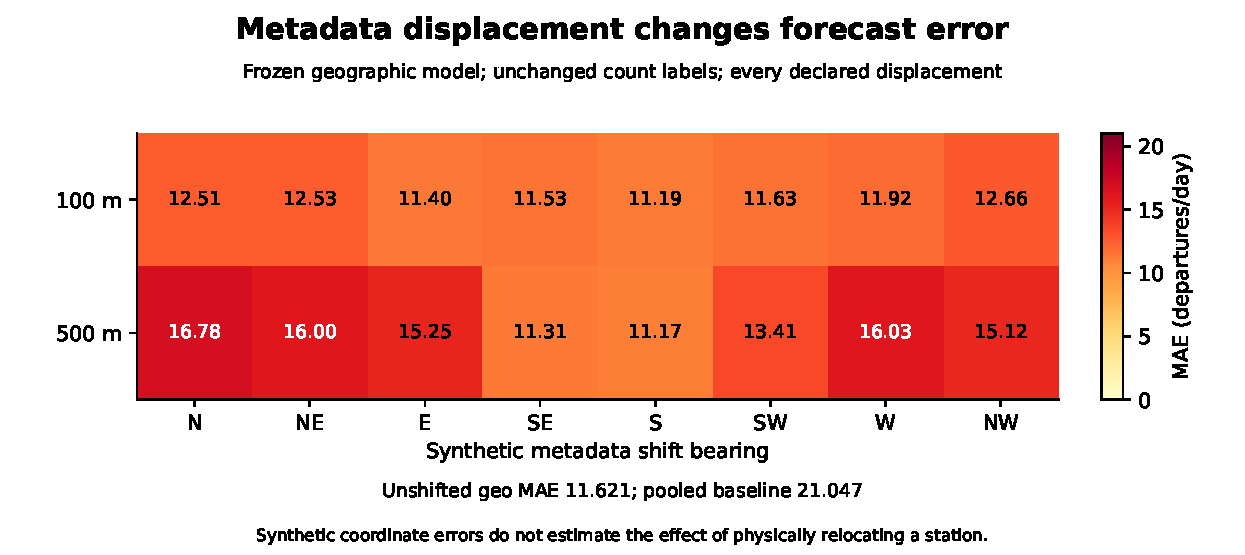
\includegraphics[width=\linewidth]{images/geography_sensitivity.pdf}\end{center}
\small Figure 3. Frozen-model metadata coordinates move 100 m or 500 m in every declared bearing while count labels remain unchanged. This tests synthetic metadata sensitivity, not an observed physical relocation.\normalsize\par

All 17 geographic cases include the unshifted reference and sixteen displacements. Each reuses the same 2,208 labels. Together with the pooled baseline they produce 39,744 held predictions, not additional independent observations. Bearing is clockwise from north. Positive change from unshifted means a worse geographic forecast.

\begin{center}\small\setlength{\tabcolsep}{4pt}
\begin{tabular}{rrrrr}\toprule
Shift (m) & Bearing (deg) & Geo MAE & Change from unshifted & Difference from pooled \\
\midrule
0 & n/a & 11.621 & 0.000 & -9.426 \\
100 & 0 & 12.510 & 0.889 & -8.537 \\
100 & 45 & 12.528 & 0.906 & -8.520 \\
100 & 90 & 11.399 & -0.222 & -9.648 \\
100 & 135 & 11.527 & -0.094 & -9.520 \\
100 & 180 & 11.190 & -0.431 & -9.857 \\
100 & 225 & 11.628 & 0.007 & -9.419 \\
100 & 270 & 11.916 & 0.294 & -9.132 \\
100 & 315 & 12.665 & 1.043 & -8.383 \\
500 & 0 & 16.782 & 5.161 & -4.265 \\
500 & 45 & 15.999 & 4.378 & -5.048 \\
500 & 90 & 15.255 & 3.633 & -5.793 \\
500 & 135 & 11.311 & -0.311 & -9.737 \\
500 & 180 & 11.173 & -0.449 & -9.875 \\
500 & 225 & 13.407 & 1.786 & -7.640 \\
500 & 270 & 16.033 & 4.411 & -5.015 \\
500 & 315 & 15.117 & 3.496 & -5.930 \\
\bottomrule\end{tabular}\end{center}
The northward 500 m case raises MAE to 16.782, while every declared aggregate case remains below the fixed pooled MAE of 21.047. These finite directions and the unchanged original labels cannot establish an actual relocation response. No displacement was used to select parameters or remove a group.

\newpage\section*{5. Uncertainty, scope and verification}
For the unshifted comparison, 1,000 resamples draw twelve held coordinate groups with replacement using seed 20261029. Every sampled index and resulting exact exported-loss difference is retained. The central empirical 2.5th--97.5th nearest-rank range for geographic-minus-pooled MAE is -15.700 to -4.198 departures/day. This is conditional finite-group resampling sensitivity, not guaranteed confidence or future coverage. Nearby groups can remain dependent; twelve groups cannot establish general spatial representativeness.

Station-ID lineage, actual opening/relocation dates and recorded coordinates are not independently surveyed. Initial screens condition on active/stable-looking first-quarter records, and later closures/reporting gaps may appear as zero published starts. Trip logs omit failed attempts and do not identify latent demand, stock or dock occupancy; prior work uses availability information for excess-demand estimation [3]. Spherical proximity omits barriers and route access. Weather, events and service operations are not modeled. The pooled baseline is not separately tuned over temporal settings. A matched-setting comparison on a new held cohort is needed to isolate geographic pooling.

Public files were posted after the measured periods. Strictly past donor indices pass under an explicitly idealized prior-day completeness assumption; actual historical input vintages and prospective feasibility remain unverified. No causal, passenger-benefit, stock, savings, true relocation, operational-readiness, peer-review or exhaustive novelty claim follows.

Nineteen fixtures cover geometry, calendar boundaries, withheld targets, donor count, distance ties/floors, weighted prediction, group loss weighting and undefined WAPE. Independent SQL histories, unit-vector geometry/displacements and fractional exported-loss checks cover 1,673,256 exact scalar fields and 477,012 numerical-tolerance checks. Prediction tolerance is absolute 1e-8, metric tolerance 1e-7 and distance tolerance 1e-8 km; these are numerical reconstruction bounds, not source or physical accuracy.

The isolated replay matches 1,643,477 fields exactly and checks 505,372 numerical fields at fixed tolerances, plus three verification documents and all 24 protected dependencies. Floating-point forecasts are exported with round-trip decimals; count-loss fractions are exact relative to those decimals. Recomputed validation configuration/scores are checked before original frozen reference bytes are restored for held use. This verifies the original frozen choice rather than selecting a new one.

The original figures have 278 actual artist-value checks, twelve map labels, sixteen annotation/contrast checks and nine hashes. Rendered-page review is separate and does not establish accessibility conformance. Source and metric checks are finite evidence, not universal correctness or independent passenger-truth audits.

\newpage\section*{6. Reproduction, source rights and next evidence}
Reproduce from the repository root using Python 3.10 and the pinned numerical/plot/PDF packages. Original per-policy runtime and shared-feature preparation are exported; timings are not a portable performance claim and variable replay times are excluded from deterministic identity.

\begin{quote}\small\begin{verbatim}
python -m pip install -r requirements.txt
python -m unittest discover -s tests -v
python src/check_reproduction.py
python src/verify_figures.py
python src/verify_paper.py
python src/verify_public_package.py
\end{verbatim}\end{quote}

Replay uses the captured coarse study inputs rather than silently fetching a later source. Original-file parsing can be repeated with the supplied verifier and privately retrieved official archives. LF text and binary attributes preserve canonical input/paper bytes on checkout. Release additionally requires scoped privacy/canonical checks, exact-head Linux success, matching tested/merged trees and an annotated remote tag.

This is a noncommercial independent analysis. The provider policy permits analysis and source material in such studies, with restrictions [2]. Public material is minimal coarse derivatives within the study; raw trip files are not hosted or distributed as a standalone dataset. Customer linkage, private rider attributes, full third-party documents, logos and implied endorsement are excluded. Source rights are not represented as public-domain or unrestricted data rights.

Before prospective use, verify station identities, geometry history, publication latency and target population. Obtain opening/relocation, bike-stock and availability observations for an actual rebalancing study. The current result supports a candidate count-transfer comparison and an evidence collection plan. Formal-publication projects, including Azure optimization, remain private.

\section*{References}\small
[1] Source provider. \href{https://citibikenyc.com/system-data}{System Data}; official JC-2024 ZIP files via \href{https://s3.amazonaws.com/tripdata/index.html}{the linked archive bucket}. Exact object/member hashes in the manifest. Accessed 29 October 2026.\par
[2] Source provider. \href{https://citibikenyc.com/data-sharing-policy}{Data Sharing Policy}. Purpose-bound noncommercial analysis/source-material scope and restrictions; raw files excluded.\par
[3] Liu X, Pelechrinis K (2021). \href{https://doi.org/10.1371/journal.pone.0252894}{Excess demand prediction for bike sharing systems}. PLoS ONE 16(6):e0252894. Availability evidence distinguishes unobserved demand from recorded trips.\par
[4] Scikit-learn official documentation. \href{https://scikit-learn.org/stable/modules/neighbors.html}{Nearest Neighbors}, regression section. Established neighbor-mean and inverse-distance concepts. The stated rolling-donor method is implemented directly here; no scikit-learn execution or novel estimator is claimed.
\end{document}
